\documentclass[12pt,a4paper]{article}
\usepackage{enumerate} %put in numbers or bullet points
\usepackage{setspace}
%\raggedright %justify the text on the left only
\usepackage{graphicx} 	% For adding pictures
\usepackage{float}
\usepackage{pdflscape}	% for landscape pages
\pagenumbering{arabic}	% Page numbers
\usepackage{fancyhdr} % add headers and footers
\usepackage{hyperref} % hyper links for references

\onehalfspacing %1.5 line spacing
\usepackage[round]{natbib} % author-year citations in round brackets

%End of preamble
%--------------------------------------------------
%Annotated thesis table of contents to accompany the continuation meeting report in September 2014
\begin{document}

\title{Thesis structure and plans for completion}
\author{}
\date{}
\maketitle


	I have started to put my thesis together. I have already completed some of the sections and the remaining work should be very manageable before my planned hand in date in January (table \ref{tab:dates}). Here I present the thesis structure with comments on the estimated length of each section, the amount of work remaining and the dates when I plan to finish full drafts of each section (table \ref{tab:dates}). 

\section{Introduction}
	There will be five subsections in the introduction. I have completed drafts of sections \ref{int_disp}, \ref{int_tenrecs} and \ref*{int_struc}. It will not take long to put the rest of the information together as I have already done a lot of the background research. I will finish writing this chapter after I have completed the analyses for chapters 2, 3 and 4. I estimate that the full chapter will be around five pages long and I will finish it before the 21st of November (table \ref{tab:dates}).


	\subsection{Patterns of morphological diversity}
		I will introduce my research within the context of other studies which are interested in understanding patterns of phenotypic variation, particularly morphological differences measured with a geometric morphometrics approach. 

	\subsection{Disparity}
		\label{int_disp}
		Leading on from my introduction about morphological diversity, I will discuss how groups which show high levels of disparity (diversity of form) are particularly interesting when it comes to understanding the factors that lead to adaptive radiations \citep{Losos2010a}. This section will be partly based on the introduction in my paper draft.  
		
	\subsection{Convergence}
		\label{int_conv}
		While disparity assesses the diversity of morphological form, morphological convergence takes the opposite approach by measuring the phenotypic similarities among distantly related species. I will include a brief summary of why convergent evolution continues to attract such great interest among researchers and the particular importance of taking quantitative approaches towards measuring degrees of convergence.
	
	\subsection{Tenrecs}
		\label{int_tenrecs}
		The background sections above will lead me in to introducing tenrecs as an example of a group which appears to show both morphological diversity and convergence with other small mammal species. In particular, I will show that tenrecs are often used as an example of both an adaptive radiation and a group which appears to be convergent with other species \citep[e.g.][]{Eisenberg1969, Soarimalala2011, Olson2013} yet these assumptions about their morphological diversity have not been tested . 
			 
	\subsection{Structure and contents of the thesis}
		\label{int_struc} 
		Finally, I will outline the remaining sections of my thesis: data collection, separate chapters for my analyses of disparity and convergence and then a general discussion chapter with future directions at the end.
%-------------------------------------------------------

\section{Data collection and processing}
	
	I'm using the same morphological data and general geometric morphometric analyses for both chapters \ref{sect_disp} and \ref*{sect_conv}. Therefore, I will combine all of this information into one data chapter to avoid later repetition. I have completed most of this chapter but there are a few additional diagrams and analyses to add. I expect the completed chapter to be approximately 25 pages (due to the number of figures and tables, not just text!) and I will finish the first draft of the chapter by the 3rd of October (table \ref{tab:dates}).

	\subsection{Data collection}
		This section includes details of the species I measured, data collected, linear measurements and methods for photographing and processing images. I have finished all of this section with the exception of creating diagrams to depict the linear measurements for skulls and limbs.

	\subsection{Geometric morphometric analyses}
		Here I describe all of my morphometric analyses including landmark choice, landmark placement and General Procrustes superimposition analyses. I have completed the analyses, diagrams and write up for all of this section.
		
	\subsection{Error checking}
		Finally, I will discuss the approaches I included in my methods to deal with potential taxonomic, identification, measurement and morphometrics errors. I have completed half of this section but I still need to run a sensitivity analysis to check the accuracy of landmark placement on my pictures. I have all of the data prepared so they will not take long to complete.

%------------------------------------------------
\section{Disparity in tenrecs compared to their closest relatives}
	\label{sect_disp}
	This chapter will be based on the paper draft which accompanies this report. It will include a brief introduction (with reference back to the disparity section  in chapter 1) and methods for how I quantified disparity within tenrecs and golden moles. The results section will be based on my draft paper and the chapter will finish with a brief discussion.
	I have almost finished this chapter, all that remains is to work on the comments I receive on the paper draft. I expect the completed chapter to be no more than six pages and I will have it finished by the 12th of September (table \ref{tab:dates}).
	

\section{Convergence among tenrecs and other small mammals}
	\label{sect_conv}
	This chapter will have the same layout as chapter \ref{sect_disp}: brief introduction with reference to section \ref{int_conv} and a description of the methods I use to quantify convergence. 
	
	I will take two approaches for quantifying convergence: estimating the amount of convergence in the tenrec phylogeny as a whole \citep{Stayton2008} and measuring the strength of convergence among specific groups of species \citep{Arbuckle2014}. These methods should be straightforward to implement because I have both the phylogenetic and morphological data prepared. 
		
	The Wheatsheaf index \citep{Arbuckle2014} measures the strength of convergence in groups which are \textit{a priori} identified to be similar. Therefore I will divide tenrecs into four separate groups and measure their morphological convergence with other small mammals. These divisions are based on the phenotypic and ecological similarities among the species and the common assumptions that tenrecs are convergent with these other groups \citep[e.g.][]{Soarimalala2011, Olson2013}. 
	
	I will compare spiny tenrecs (\textit{Echinops, Setifer, Tenrec} and \textit{Hemicentetes}) to hedgehogs, gymnures and solenodons while mole-like tenrecs (\textit{Oryzorictes}) will be compared to moles and golden moles. Most tenrecs (\textit{Microgale} genus and \textit{Geogale aurita}) are shrew-like so I will compare these species to my morphological measurements of shrews. I will also try to compare convergence within a semi-aquatic grouping of \textit{Limnogale} and \textit{Potamogale} tenrecs along with gymnures and water shrews although I may not have a sufficient sample size for this analysis. 
	
	The initial outputs of my convergence analyses will be PCA plots of morphospace occupation by each family of small mammals. Figure \ref{fig:skdors_pca} is an example PCA plot for the analysis of skulls in dorsal view. These plots give a visual representation of the phenotypic similarities among my species.

	I will use these plots to calculate morphological distance matrices among species pairs. I will combine these morphological differences with phylogenetic distance matrices to generate an overall measure of the amount of convergence within the tenrec family \citep{Stayton2008} and the strength of convergence between sub-groups of tenrecs and other small mammal species \citep{Arbuckle2014}.
	
	I will finish the chapter with a brief discussion of the implications of my results although most of this information will be included in my final discussion chapter. I expect the completed chapter to be no more than eight pages and I will finish a full draft by the 31st of October (table \ref{tab:dates}).
	

%----------------------------------------------
  \begin{figure}[H]
	\centering
	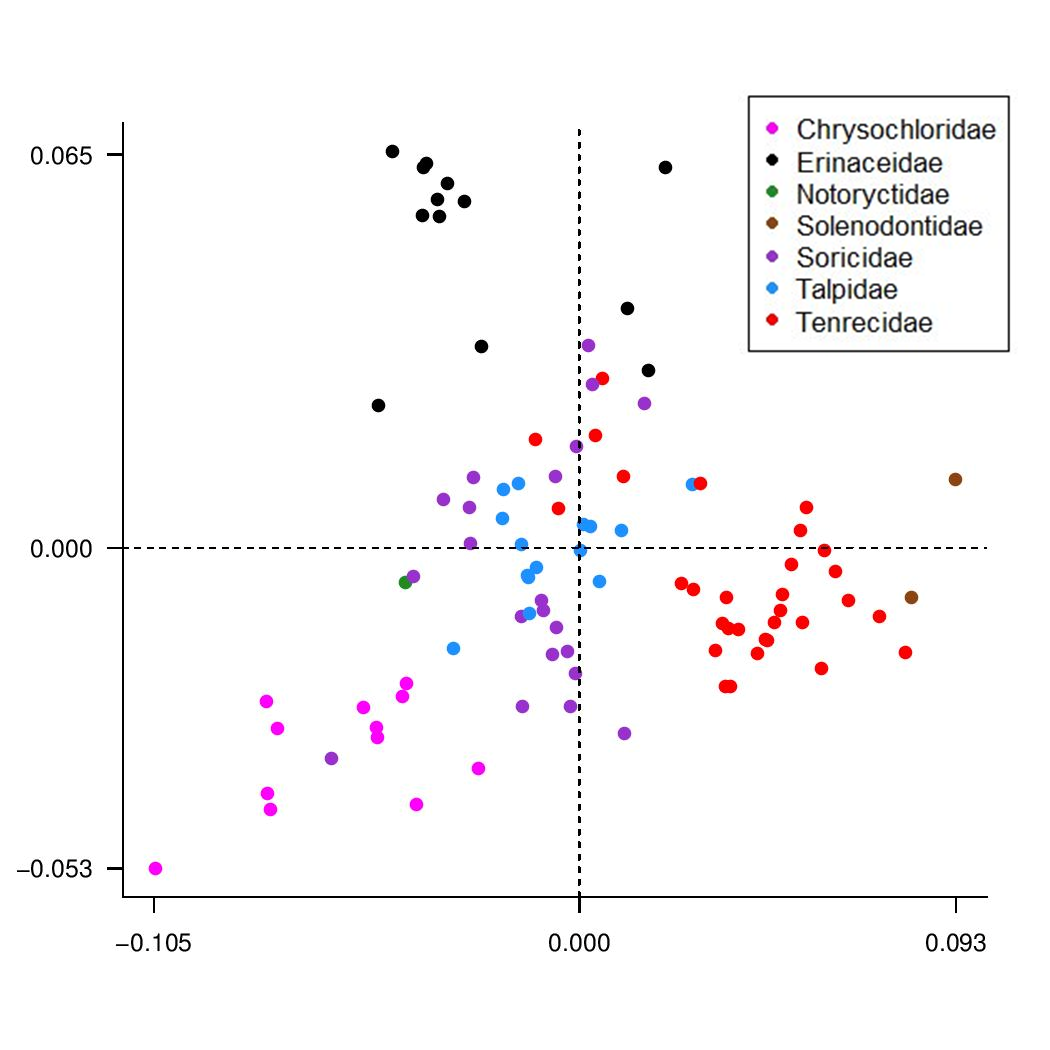
\includegraphics[width=\textwidth, height=\textheight, keepaspectratio=true]{skdors_allfam_PCA_legend.png}
		\caption{Morphospace (principal components plot) of the Procrustes-superimposed shape coordinates for skulls in dorsal view. Each point represents the average skull shape of an individual species and points are coloured by Family.}
	\label{fig:skdors_pca}
  \end{figure}

%---------------------------------------------------------

\section{Discussion}
	
	Here I will summarise my findings and interpret the results within the context of what they tell us about morphological diversity within tenrecs and the similarities among tenrecs and other small mammal species. I will also highlight the importance of taking a quantitative approach to studies of evolutionary diversity among species groups. In particular I will stress the need to apply existing methods to new groups of species which are usually not as well studied as the groups that are used to develop such metrics. 
	I will follow this overall discussion with a clear recognition of the potential issues associated with my approach including possible biases introduced by some measurements and an acknowledgement that cranial morphology is only one aspect of phenotypic variation.
	
	The rest of the chapter will be suggestions for future research directions based on some of the original plans that I had made for continuing with the PhD. These will include the possibility of applying multiple metrics for measuring convergence \citep[e.g.][]{Ingram2013, Segar2013, Harmon2005}, analyses of ecological similarities to test whether there are correlations between ecological and phenotypic convergence \citep[e.g.][]{Moen2013} and the need to measure the functional importance and `adaptiveness' of convergent traits \citep{Losos2010}. I will also include a brief mention of my unsuccessful fieldwork experiments for testing echolocatory capabilities in \textit{Microgale} tenrecs and the potential for future studies of behavioural convergences among tenrecs and other small mammals.

	I expect this chapter to be around eight pages and I will aim to finish it on the 12th of December (table \ref{tab:dates}).


%--------------------------------------------------------------
%Table with dates for completion

	\begin{table}[h]			
	\caption
		{Timetable for completion of my thesis.}
	\centering
	%Timetable for thesis completion


\begin{tabular}[t]{l l l l }		
\hline
\textbf{Task} & \textbf{Start} & \textbf{End} & \textbf{No. of weeks} \\ 
\hline
%-----------------------------------
Finish disparity chapter & 1st September & 12th September & 2 \\
%-----------------------------------
Error checking analysis & 15th September & 26th September & 2 \\
%-----------------------------------
Finish data chapter & 29th September & 3rd October & 1 \\
%-----------------------------------
Convergence analysis & 6th October & 24th October & 3 \\
%-----------------------------------
Convergence write up & 27th October & 31st October & 1 \\
%-----------------------------------
Introduction & 3rd November & 21st November & 3 \\
%-----------------------------------
Discussion & 24th November & 12th December & 3 \\
%-----------------------------------
Address remaining comments  & 5th January & 28th January & 3.5 \\
%-----------------------------------
&&&\\
%-------------------------
\textbf{Submit thesis} & & \textbf{30th January} & \\ 
\hline
\end{tabular} 
	\label{tab:dates}  
	\end{table}
%-------------------------------------------------------

\bibliographystyle{jeb}
\bibliography{refs_thesis} 
\end{document}